\ifcase 1  % choose 0=slides, 1=article, 2=refart
   \documentclass[aspectratio=169,ignorenonframetext,9pt]{beamer}
\or\documentclass[a4paper,11pt]{article}
   \usepackage{url,beamerarticle}
\or\documentclass[a4paper,11pt]{refart}
   \let\example\relax
   \usepackage{url,beamerarticle}
\fi

\ifcase 0  % choose a theme like these
    % \usetheme{boxes}
    \usetheme{Boadilla}
    % \usetheme{Goettingen}% I recommend
    % \usetheme{Singapore}
    % \usetheme{Pittsburgh}
    % \usetheme{Madrid}
    % \usetheme{Warsaw} % common choice, but often poor
\fi

\usepackage{algorithm,algorithmicx}
\usepackage{graphicx,pgfplots,parskip}
\usepackage{amsmath,amsfonts,amssymb,amsthm,epsfig,epstopdf,url,array}
\usepackage{cite}




\theoremstyle{plain}
\newtheorem{thm}{Theorem}[section]
\newtheorem{lem}[thm]{Lemma}
\newtheorem{prop}[thm]{Proposition}

\theoremstyle{definition}
\newtheorem{defn}{Definition}[section]
\newtheorem{conj}{Conjecture}[section]
\newtheorem{exmp}{Example}[section]
\newtheorem{algo}{Algorithm}[section]


\title{BSTERGM: Bayesian Separable-Temporal Exponential family Graph Models}
\author{Choi, Seokjun}
\date{14 Dec. 2020}


\begin{document}

\begin{frame}
\maketitle
\end{frame}


\begin{abstract}
Separable Temporal Exponential Random Graph Models (STERGMs) are useful models to describe changes in dynamic networks' structures evolving over time. 
The Bayesian-inference based approach for the model, however, had not been developed yet. 
In this paper, I propose the Bayesian STERGMs (BSTERGMs): STERGMs with the Bayesian setting, and I illustrate the computational algorithm that generates posterior samples from the model dealing with the doubly-intractable constant problem. 
Furthermore, I show the interpretability of the model in the Bayesian context.

\end{abstract}


% \begin{frame}{Outline}
% \tableofcontents
% \end{frame}

\section{Introduction}
Nowadays, new kinds of data having special forms emerge in many field.
These new data are not confined by a series of values of real numbers as traditional data are in the past. 
The data may have non-number type of value, special structure, or even integrated different type of values with model-specific relation.
These data are called complex data, and an attention of statistical analysis on the data increases over time.

As one form of the complex data, networks get highlighted attention among complex data for statistical analysis.
Many phenomena can be represented by some relational structure, and the structure can be expressed effectively
by a form of a network. For example, social networks including both offline and online can be thought as a sort of networks.
In this view, some social aspects of relation between actors can be modeled with an object of social science
including an analysis of power structure and a summary of intimacy structure on given group.
Not only that, application to a transmitted disease leads a modeling using real data in epidemiology.

Since statistical models on network provide not only lots of possibility of application but also
interesting and useful features on observed network, statistical models have important role.
The statistical model gives information about local relations like formation or dissolution between
two actors as well as global features of the whole network such as probability that a specific structure
realizes. Not only that, the statistical models investigate a complex behavior of network including
how the global features of an observed network may be related to local network structure.
During the investigation, statistical model can capture existing dependency on a given network
and provide a tool to understand what certain structural features are more common on rare.

Exponential-family random graph models(ERGMs) may be the most useful tools to analyze cross-sectional networks and their dependencies.
\cite{RN117}, \cite{RN123}, \cite{RN124} and \cite{RN122} proposed the models and apply them to analyze dependent structures,
and the Bayesian approaches of the models were started by \cite{RN115} and \cite{RN116}.
In the ERGMs, The dependencies are captured using a series of local features called network statistics from classical graph-theory.
Since these models play important role in this paper, I will introduce more precisely.

Next natural question is a way to model a network sequence, or the evolution of network over time.
For instance, one may want to model social network structures for 1 year, or
simulation of a disease infection based on the sequential observations in the past.
The first exploration applying ERGMs was \cite{RN109}. 
After them, a notable contributions were of \cite{RN125} and \cite{RN126}, the Temporal ERGMs(TERGMs).
In the TERGM, ERGMs are used by modelling the transition probability between times.
Moreover, \cite{RN93} extend the TERGMs to the Separable Temporal ERGMs(STERGMs), considering an
separation between duration - how long ties tend to last - and incidence - the rate at which new ties are formed -
from prevalence - for example, the total number of ties - of the network properties.
Imposing a conditional independence condition between the duration and incidence,
the models can be extended effectively using similar fitting methods with TERGMs
without adding much complexity.

Although the STERGMs give us strength when it comes to interpret the fitted parameter,
a Bayesian approach for the STERGMs has not been conducted. It is partly because of a hardship
coming from the huge computation in a parameter estimation method for the model.
Nonetheless, the Bayesian approach of STERGMs provides the statistical inference method
following the standard Bayesian way, so the approach has huge advantage of convenience
for statistical works for fitted parameter and predictions to next time network structure.
Thus, in this paper, I specify the bayesian separable temporal exponential random graph models(BSTERGMs)
and propose a fitting algorithm for the model parameter. 
I also discuss ways of inference, the diagnostics procedure, and checking the goodness of fit.

In chapter 2, I review the background meterials including ERGMs, BERGMs, TERGMs, and STERGMs,
and in chapter 3, I show the detail setting of BSTERGMs. In chapter 4, I propose the fitting method for BSTERGM.
In chapter 5, I explain ways to conduct diagnostics, statistical inference, and goodness of fit check.
In chapter 6, I illustrate an application of BSTERGMs to network data of scholars and faculty
from the UCLA medical working project team. Finally, I discuss some extension and 
ways to supplement the BSTERGM further for future research.


\section{Background}
\subsection{Random graphs}
For statistical analysis on relations between subjects of data,
I will introduce terminologies and notations for denoting components related to networks, 
which are a representation of these type of data.

We say each subject on the data to a node. They are same as a vertex in graph theory.
In addition, we say a tie joining two nodes to an edge. A tie can be directed or not.
These two components have fundamental role describing the data.
Define a graph or a network to $y=(V,E)$, where $V$ is a set of node and $E$ is a set of edges of a network.

For simplicity, I will deal with a situation without weight on each node or edge.
Then, a graph $y$ can be represented by simpler form.
Assume that the number of node $n\in \mathbb{N}$ on data is given.
Then, for $\mathcal{B}=\{0,1\}$,
the set $\mathcal{Y} \subset \mathcal{B}^{n^2}$ is a set of graphs of $n$ nodes.
Now, a graph $y \in \mathcal{Y}$ can be represented by a $n \times n$ binary matrix
with elements $y_{ij}=1$ if there is a tie from $i$-th node to $j$-th node,
otherwise $y_{ij}=0$.

If edges of $y$ have directions, then $y$ is called a directed graph. Otherwise, $y$ is called a undirected graph.
These are obvious that, for given $n\in \mathbb{N}$,
$|\mathcal{Y}|=2^{n(n-1)}$ if $\mathcal{Y}$ is the set of all directed graphs not permitting self-connecting edges,
and $|\mathcal{Y}|=2^{n(n-1)/2}$ if $\mathcal{Y}$ is the set of all graphs of undirected one.
Thus, the size of $\mathcal{Y}$ grows exponentially when n increases.

I extend the concept of graphs to be able to describe a situation that connections among nodes are random.
Let $\Omega$ be an event set of all possible connected situations among given nodes.
We say $Y: \Omega \to \mathcal{Y}$ is a random variable for a graph, or a random graph.
For a random graph $Y \in \mathcal{Y}$, denote the edge between i-th node and j-th node by $Y_{ij}$ for $i,j=1,2,...,n$
satisfying $Y_{ij}=1$ if the edge is connected. Otherwise, $Y_{ij}=0$.
Note that the $Y_{ij}$s are also random variables.

Let me notate a realization of random graph by $y$ and its edges by $y_{ij}$ for $i,j=1,2,...,n$.


\subsection{ERGMs: Exponential random graph models}
From the definition of random graph, one of the natural questions is 
how we can model a distribution on $\mathcal{Y}$.
As a answer, the Exponential random graph models (ERGMs) (\cite{RN123} and \cite{RN122})
gives a classical but 
flexible scheme to model for time-invariant networks represented as a single directed or undirected graph.
Moreover, ERGMs provide a statistical approach to the systematic exploration of several local features simultaneously and 
how these local structures interact to form a global network.

Specifically, following the notation of previous section,
let $\mathcal{Y}$ be a set of random graphs with $n$ nodes and $Y \in \mathcal{Y}$ be a random graph.
Set a distribution on $\mathcal{Y}$ to
    \[P(Y=y;\theta) = \frac{exp(\theta^{T}s(y))}{c(\theta)}\]
for some $\theta\in\mathbb{R}^p$,
where $s(y)\in\mathbb{R}^p$ is a vector which is part of y's sufficient network statistics,
and $c(\theta)\in\mathbb{R}$ is a normalizing constant satisfying $c(\theta)=\sum_{y\in\mathcal{Y}}exp(\theta^{T}s(y))$.
Models which have such a form called the ERGMs.

Note that the form of the right-hand side is the canonical form of exponential family distributions.
That is why the model is called exponential. Moreover, observe that the normalizing constant cannot be directly calculated
because the size of $\mathcal{Y}$ grows exponentially as $n$ grows.
Thus in real data analysis, the calculation of $c(\theta)$ should be avoided.
For more detail of fitting algorithm, see \cite{RN104} the detail on fitting algorithm using MCMCMLE.
You can also see \cite{RN100} addressing the ergm package in R with the MCMCMLE or the classic method using psudolikelihood.


\subsection{BERGMs: Bayesian ERGMs}
\cite{RN115} and \cite{RN116} extend ERGMs to bayesian setting. Putting prior $p(\theta)$ to the parameter $\theta$, the model becomes
\[p(\theta|y)=\frac{p(y|\theta)p(\theta)}{p(y)}=\frac{exp(\theta^T s(y))}{c(\theta)}\frac{p(\theta)}{p(y)}\]

Observe that not only $c(\theta)$ but also the $p(y)$ cannot be evaluated directly
because of the difficulty of summation when $n$ grows and of integration of $p(y)$.
Moreover, the constant depends on the parameter $\theta$, so ordinary MCMC technique cannot be used.
This situation is said to doubly-intractable constant problem(\cite{RN119}), and causes serious challenge to estimate the parameter vector $\theta$.
Thus, The estimation of $\theta$ needs more advanced algorithm than the standard MCMC procedure.
The solution of Caimo and Friel is using the exchange algorithm. See \cite{RN115} for details of fitting methods of BERGMs
and \cite{RN127} for the exchange algorithm.


\subsection{TERGMs: Temporal Exponential family Random Graphs Models}
Let's consider a sequence of random graph $\{Y_1, Y_2, ..., Y_T\} (T\in\mathbb{N})$ and assume that
we are interested in the dynamics or evolution of the network sequence.
The temporal Temporal Exponential family Random Graphs Models(TERGMs)
proposed by \cite{RN125} and \cite{RN126}
is a model for our interest if we permit a Markov assumption
\[P(Y_2,Y_3,...,Y_T|Y_1)=P(Y_2|Y_1)P(Y_3|Y_2)...P(Y_T|Y_{T-1})\]
and focus on the transition probability along index of the sequence.
For convenience, I refer the index as a time.

Specifically, let $\mathcal{Y}$ be a set of graphs with $n$ nodes. 
Let $Y_1=y_1 \in \mathcal{Y}$ be given and $Y_2,...,Y_T (T\in\mathbb{N})$ be random graphs in $\mathcal{Y}$.
Set a distribution on $\mathcal{Y}\times ... \times \mathcal{Y}$ ($T-1$ folds) to
\[P(Y_t=y_t|Y_{t-1}=y_{t-1};\theta) = \frac{exp(\theta^{T}s(y_t, y_{t-1}))}{c(\theta, y_{t-1})}\]
where $t=2,...,T$, $\theta\in\mathbb{R}^p$,
sufficient network statistics $s(y_t, y_{t-1})\in\mathbb{R}^n$,
and a normalizing constant $c(\theta, y_{t-1})=\sum_{y\in\mathcal{Y}}exp(\theta^{T}s(y, y_{t-1}))$.
Models which have a such form called the TERGMs.

The estimation of $\theta$ can be performed by MCMCMLE,
but the estimation suffers severe degeneracy problem.
Furthermore, When we interpret the estimated TERGMs parameters,
we cannot separate the generation and duration because
the higher value of $\theta$ increases both.
These raise demand for modified models to remedy the degeneracy and enable separable interpretation.

\subsection{STERGMs: Separable-Temporal Exponential family Random Graphs Models}
One solution to remedy the problems of TERGMs is 
the Separable-Temporal Exponential family Random Graphs Models, or simply STERGMs. %ref
The key idea is to separate the formation models and dissolution model
for decoupling an effect on edge's duration of model parameter from edge's incidence
when setting a distribution on $\mathcal{Y}\times ... \times \mathcal{Y}$ ($T-1$ folds, $T\in\mathbb{N}$),
where $\mathcal{Y}$ is a set of graphs with given $n$ nodes.

Precisely,
Let $Y_1=y_1 \in \mathcal{Y}$ be given and $Y_2,...,Y_T$ be random graphs (on $\mathcal{Y}$).
Let $\mathcal{Y}^+|_t$ be a subset of $\mathcal{Y}$ consisting all graphs which have equal or additional edges comparing to $y_{t-1}$.
Likewise, let $\mathcal{Y}^-|_t$ be a subset of $\mathcal{Y}$ consisting all graphs which have equal or sparse edges comparing to $y_{t-1}$.
Next, for $Y_t^+: \Omega \to\mathcal{Y}^+|_t$, $Y_t^-: \Omega \to\mathcal{Y}^-|_t$, $y_t^+ \in \mathcal{Y}^+|_t$ and $y_t^- \in \mathcal{Y}^-|_t$, set
\[P(Y_t^+=y_t^+|Y_{t-1}=y_{t-1};\theta^+) = \frac{exp((\theta^+)^{T}s(y_t^+, y_{t-1}))}{c(\theta^+, y_{t-1})}\]
\[P(Y_t^-=y_t^-|Y_{t-1}=y_{t-1};\theta^-) = \frac{exp((\theta^-)^{T}s(y_t^-, y_{t-1}))}{c(\theta^-, y_{t-1})}\]
for some $\theta^+,\theta^-\in\mathbb{R}^p$, $s(y_t^+, y_{t-1}), s(y_t^-, y_{t-1})\in\mathbb{R}^n$, which are parts of sufficient network statistics,
and normalizers $c(\theta^+, y_{t-1})=\sum_{y^+\in\mathcal{Y}^+}exp((\theta^+)^{T}s(y^+, y_{t-1}))$, 
and $c(\theta^-, y_{t-1})=\sum_{y^-\in\mathcal{Y}^-}exp((\theta^-)^{T}s(y^-, y_{t-1}))$.

Then, defining operations $+,-$ on $\mathcal{Y}$ following the edgewise boolean algebra,
(For detail, Define binary operations on the edge values $\{0,1\}$ by $+$ and $-$ 
by $1+1=1, 1+0=0+1=1, 0+0=0$ and $1-1=0, 1-0=1, 0-1=0, 0-0=0$) 
set the combined network $y_t$ to
\[y_t=y_t^+ - (y_{t-1} - y_t^-) = y_t^- + (y_t^+ - y_{t-1})\]

Additionally, assume the first-order Markov assumption
\[P(Y_2,...,Y_T|Y_1)=P(Y_2|Y_1)...P(Y_T|Y_{T-1})\]
and the conditional independence between $Y_t^+$ and $Y_t^-$ for all $t=2,...,T$, called the separability.
Then we get
\[P(Y_t=y_t|Y_{t-1}=y_{t-1};\theta^+,\theta^-)=P(Y_t^+=y_t^+|Y_{t-1}=y_{t-1};\theta^+) P(Y_t^-=y_t^-|Y_{t-1}=y_{t-1};\theta^-)\]
Models which have a such form called the STERGMs.



\subsection{Network Statistics for ERGMs and derived models}
Now, I briefly discuss the terms of network statistics.
As a usual, $s(y)$ of ERGMs or $s(y_{t}^.,y_{t-1})$ of TERGMs and STERGMs would 
reflect the structure of given network without identifying each node index.
Common candidates of the statistics are here.


Let $y\in\mathcal{Y}$ and $n\in\mathbb{N}$ be the number of nodes of $y$.
The simplest candidate is the number of edges, denoted by $|y|$.
Following \cite{RN104}, common candidates are distributions defined by some sense of structure of given graph.
For a given $i, 1\leq i \leq n-1$, $D_i(y)$ is defined to be a number of nodes in y whose the number of edges incident to the node equals $i$,
and called $i$-th order node degree distribution. 
For a given $i, 1\leq i \leq n-2$, $P_i(y)$ is defined to be a number of dyads $(j,k), 1\leq j,k \leq n$
in y whose $j$ and $k$ have nodes connected by an edge each other and they share exactly $i$ connected nodes in common,
and called $i$-th order edgewise shared partner distribution.
Note that, the bundle of all order of node degree distribution and all order of edgewise shared partner distribution,
\[(D_1(y),D_2(y),...,D_{n-1}(y),P_1(y),P_2(y),...,P_{n-2}(y))\] 
forms sufficient statistics of a graph.
And there are relation that
\[n=D_0(y)+D_1(y)+...+D_{n-1}(y)\]
and
\[|y|=P_0(y)+P_1(y)+...+P_{n-2}(y)=\frac{1}{2}\sum_{i=1}^{n-1} iD_i(y)\]


A function of the sufficient statistics can be candidates for the model statistics.
\cite{RN128} proposed graph statistics including $k$-star $S_k(y)$ for $1\leq k \leq n-1$ and $k$-triangles $T_k$ for $1\leq k \leq n-2$.
The $k$-star consists of a node together with a set of $k$ of its connected nodes,
and the $k$-triangle consists of $k$ triangles that share one common edge.
They can be expressed by the definition of node degree distributions and edgewise shared partner distributions,
\[S_1 = |y|, 
S_k = \sum_{i=1}^{n-1} \binom{i}{k} D_i(y), k\geq 2\]
and
\[T_1 = \frac{1}{3}\sum_{i=1}^{n-2} iP_i(y),
T_k = \sum_{i=1}^{n-2} \binom{i}{k} P_i(y), k\geq 2\]

Another interesting statistics are geometrically weighted value of distributions defined by
\cite{RN118},\cite{RN104},\cite{RN128} and \cite{RN103}.
For example, geometrically weighted (node) degree with parameter $\tau$ is defined by
\[GWD(y;\tau)=e^{\tau} \sum_{k=1}^{n-2} (1-(1-e^{-\tau})^k)D_k(y)\]
and geometrically weighted shared partner distribution with parameter $\tau$ is defined by
\[GWESP(y;\tau)=e^{\tau} \sum_{k=1}^{n-2} (1-(1-e^{-\tau})^k)P_k(y)\]


In the context of temporal models, parameters in the model take two network as a arguments like $s(y_t,y_{t-1})$.
One of common choices for these statistics is the bundle of sufficient statistics of first argument $y_t$.
Another common choice is using a difference, $s(y_t,y_{t-1})=s'(y_t)-s'(y_{t-1})$ where $s'$ is a network statistics of given network.
Although there are lots of other statistics related to ERGMs, I omit them and end this subsection here.
If you need, see \cite{RN107} for the ERGMs, and \cite{RN125}'s chapter 2.1 for temporal the ERGMs.


\section{Bayesian STERGMs}
A goal is to convert the STERGMs to the Bayesian setting.
With priors $p(\theta^+),p(\theta^-)$ over $\theta^+,\theta^-$,
the Bayesian model for the STERGMs can be made. I call this model Bayesian Separable Temporal Exponential family Random Graph Models,
or the BSTERGMs. More explicitly, for given the number of nodes $n$, let $Y_1=y_1 \in \mathcal{Y}$ be given and $Y_2,...,Y_T$ be random graphs (of $\mathcal{Y}$).
As the STERGMs, define $\mathcal{Y}^+|_t$, $\mathcal{Y}^-|_t$ be subsets of $\mathcal{Y}$ consisting all graphs which have equal or additional edges comparing to $y_{t-1}$,
and which have equal or sparse edges comparing to $y_{t-1}$ respectively.
Then, for $Y_t^+$ of $\mathcal{Y}^+|_t$ and $Y_t^-$ of $\mathcal{Y}^-|_t$, $y_t^+ \in \mathcal{Y}^+|_t$ and $y_t^- \in \mathcal{Y}^-|_t$, set
\[P(Y_t^+=y_t^+|Y_{t-1}=y_{t-1};\theta^+) = \frac{exp((\theta^+)^{T}s(y_t^+, y_{t-1}))}{c(\theta^+, y_{t-1})}\]
\[P(Y_t^-=y_t^-|Y_{t-1}=y_{t-1};\theta^-) = \frac{exp((\theta^-)^{T}s(y_t^-, y_{t-1}))}{c(\theta^-, y_{t-1})}\]
for some $\theta^+,\theta^-\in\mathbb{R}^p$, $s(y_t^+, y_{t-1}), s(y_t^-, y_{t-1})\in\mathbb{R}^n$, which are parts of sufficient network statistics,
and normalizers $c(\theta^+, y_{t-1})=\sum_{y^+\in\mathcal{Y}^+}exp((\theta^+)^{T}s(y^+, y_{t-1}))$, 
and $c(\theta^-, y_{t-1})=\sum_{y^-\in\mathcal{Y}^-}exp((\theta^-)^{T}s(y^-, y_{t-1}))$.

Then, with the edgewise boolean algebra, set the combined network $y_t$ to
\[y_t=y_t^+ - (y_{t-1} - y_t^-) = y_t^- + (y_t^+ - y_{t-1})\]

and assume that the first-order Markov property
\[P(Y_2,...,Y_T|Y_1)=P(Y_2|Y_1)...P(Y_T|Y_{T-1})\]
and the conditional independence(separability) between $Y_t^+$ and $Y_t^-$ for all $t=2,...,T$.
Then we get
\[\theta^+ \sim p(\theta^+), \theta^- \sim p(\theta^-)\]
\[P(Y_t=y_t|Y_{t-1}=y_{t-1};\theta^+,\theta^-)=P(Y_t^+=y_t^+|Y_{t-1}=y_{t-1};\theta^+) P(Y_t^-=y_t^-|Y_{t-1}=y_{t-1};\theta^-)\]

The purpose of Bayesian inference is to get information of the posterior distribution of $\theta^+,\theta^-$.
By the Bayes rule, the posterior can be expressed by
\[P(\theta^+,\theta^-|y_t, y_{t-1}) = \frac{P(Y_t^+=y_t^+|y_{t-1},\theta^+) P(Y_t^-=y_t^-|y_{t-1},\theta^-)P(\theta^+),P(\theta^-)}{c(\theta^+,y_{t-1})c(\theta^-,y_{t-1})p(y_t, y_{t-1})} \]
where $y_t=y_t^+ - (y_{t-1} - y_t^-) = y_t^- + (y_t^+ - y_{t-1})$ as set above.

Note that, the BSTERGMs also have similar kinds of problems of the BERGMs.
The normalizing constants $c(\theta^+,y_{t-1})$, $c(\theta^-,y_{t-1})$ practically cannot be computed because we need to sum up too many terms.
The constants are doubly intractable: they depend on $\theta^+$,$\theta^-$, the parameters of a model.
Thus, we cannot use an ordinary MCMC algorithm to get the posterior sample in this model,
because the constant part remains when calculating the MCMC ratio.


\section{Estimation}

Suppose that a sequence of graph samples $y_1,...,y_T$ is observed.
(then, $y_2^+,...,y_T^+$ and $y_2^-,...,y_T^-$ are uniquely determined.) 
Then how can we find the posterior distribution of $\theta^+,\theta^-$ with the observation using the BSTERGMs?
To solve the doubly-intractable constant problem, I propose an novel algorithm using the exchange algorithm,
one of the special MCMC techniques by \cite{RN127}, extending the algorithm of the BERGMs'(\cite{RN115}).
Although MCMC types of approach cannot give an analytic expression of posterior distribution,
it gives posterior samples as much as we want, and using the samples we can conduct statistical inference on given data.

The key idea is running two MCMC chain to make independent sample to cancel the constant parts
when calculating the MCMC accept-reject ratio.
As a motivation, consider the ordinary MCMC ratio for $m$-th MCMC iteration in the BSTERGMs context 
to show doubly intractable constant problem explicitly.

With symmetric proposal distribution,
\[\pi_{ordinary} = \frac{P(y_t^+|y_{t-1},\theta_*^+)P(y_t^-|y_{t-1},\theta_*^-)p(\theta_*^+)p(\theta_*^-)}
{P(y_t^+|y_{t-1},\theta_{m-1}^+)P(y_t^-|y_{t-1},\theta_{m-1}^-)p(\theta_{m-1}^+)p(\theta_{m-1}^-)}\]
where $\theta^*$ is proposed parameter in an iteration of MCMC.
Plugging specific model form to above equation,
\[\pi_{ordinary} = \frac{\frac{exp(\theta_*^+ s(y_t^+,y_{t-1}))}{c(\theta_*^+, y_{t-1})} \frac{exp(\theta_*^- s(y_t^-, y_{t-1}))}{c(\theta_*^-, y_{t-1})} p(\theta_*^+)p(\theta_*^-)}
    {\frac{exp(\theta_{m-1}^+ s(y_t^+, y_{t-1}))}{c(\theta_{m-1}^+, y_{t-1})} \frac{exp(\theta_{m-1}^- s(y_t^-, y_{t-1}))}{c(\theta_{m-1}^-,y_{t-1})} p(\theta_{m-1}^+)p(\theta_{m-1}^-)}\]
Since each c depends on unique subscript of $\theta$ respectively, the constants are not canceled out.

If we can generate simulated samples $y_{ex}|y_{t-1},\theta_{m-1}$ and $y_{ex}|y_{t-1},\theta_*$ and
calculate their probability following the BSTERGMs, this situation can be resolved.
At this point, applying the key idea mentioned above, multiply the probability terms in order to exclude the constant terms.
Then we get the exchange algorithm's ratio,
\[\pi = \frac{P(y_t^+|y_{t-1},\theta_*^+)P(y_t^-|y_{t-1},\theta_*^-)p(\theta_*^+)p(\theta_*^-)P(y_{ex}^+|y_{t-1},\theta_{m-1}^+)P(y_{ex}^-|y_{t-1},\theta_{m-1}^-)}
{P(y_t^+|y_{t-1},\theta_{m-1}^+)P(y_t^-|y_{t-1},\theta_{m-1}^-)p(\theta_{m-1}^+)p(\theta_{m-1}^-)P(y_{ex}^+|y_{t-1},\theta_*^+)P(y_{ex}^-|y_{t-1},\theta_*^-)}\]

\[=\frac{\frac{exp(\theta_*^+ s(y_t^+,y_{t-1}))}{c(\theta_*^+, y_{t-1})} \frac{exp(\theta_*^- s(y_t^-, y_{t-1}))}{c(\theta_*^-, y_{t-1})} p(\theta_*^+)p(\theta_*^-)}
{\frac{exp(\theta_{m-1}^+ s(y_t^+, y_{t-1}))}{c(\theta_{m-1}^+, y_{t-1})} \frac{exp(\theta_{m-1}^- s(y_t^-, y_{t-1}))}{c(\theta_{m-1}^-,y_{t-1})} p(\theta_{m-1}^+)p(\theta_{m-1}^-)}
\frac{\frac{exp(\theta_{m-1}^+)s(y_{ex}^+,y_{t-1})}{c(\theta_{m-1}^+, y_{t-1})}\frac{exp(\theta_{m-1}^- s(y_{ex}^-,y_{t-1}))}{c(\theta_{m-1}^-, y_{t-1})}}
{\frac{exp(\theta_*^+ s(y_{ex}^+,y_{t-1}))}{c(\theta_*^+,y_{t-1})} \frac{exp(\theta_*^- s(y_{ex}^-,y_{t-1}))}{c(\theta_*^-,y_{t-1})}}\]

\[=\frac{exp(\theta_*^+ s(y_t^+,y_{t-1})) exp(\theta_*^- s(y_t^-, y_{t-1}))}{exp(\theta_{m-1}^+ s(y_t^+, y_{t-1}))exp(\theta_{m-1}^- s(y_t^-, y_{t-1}))}
\frac{exp(\theta_{m-1}^+ s(y_t^+, y_{t-1}))exp(\theta_{m-1}^- s(y_{ex}^-,y_{t-1}))}{exp(\theta_*^+ s(y_{ex}^+,y_{t-1}))exp(\theta_*^- s(y_{ex}^-,y_{t-1}))}
\frac{p(\theta_*^+)p(\theta_*^-)}{p(\theta_{m-1}^+)p(\theta_{m-1}^-)}\]

% \[=exp((\theta_*^+ - \theta_{m-1}^+)s(y_t^+,y_{t-1}) + (\theta_*^- - \theta_{m-1}^-)s(y_t^-,y_{t-1})
% -(\theta_*^+ - \theta_{m-1}^+)s(y_{ex}^+,y_{t-1}) - (\theta_*^- - \theta_{m-1}^-)s(y_{ex}^-,y_{t-1}))
% \frac{p(\theta_*^+)p(\theta_*^-)}{p(\theta_{m-1}^+)p(\theta_{m-1}^-)}\]

\[=exp((\theta_*^+ - \theta_{m-1}^+)(s(y_t^+,y_{t-1}) - s(y_{ex}^+,y_{t-1}))(\theta_*^- - \theta_{m-1}^-)(s(y_t^-,y_{t-1}) - s(y_{ex}^-,y_{t-1})))
\frac{p(\theta_*^+)p(\theta_*^-)}{p(\theta_{m-1}^+)p(\theta_{m-1}^-)}\]

The last expression shows that all constants are canceled out.
This finding leads us to the fitting algorithm for the BSTERGMs using the exchange algorithm.


\begin{algo}[the main chain]
Let $y_1,...,y_T$ be given. For $m=1,...,M$,
\begin{enumerate}
    \item Propose candidates $\theta_*^+,\theta_*^-$ from a proposal distribution $\epsilon(.|\theta_{m-1}^+,\theta_{m-1}^-)$.
    \item Select a lag $(t-1,t)$ randomly on $2 \leq t \leq T$.
    \item Generate an exchange graph $y_{ex} \in\mathcal{Y}|_t$ (with $y_{ex}^+, y_{ex}^-$) at the $\theta_*^+,\theta_*^-$.
    \item Calculate network statistics $s(y_t^+,y_{t-1}), s(y_{ex}^+,y_{t-1}), s(y_t^-,y_{t-1}), s(y_{ex}^-,y_{t-1})$.
    \item Calculate the exchange MCMC ratio $\pi$ at the lag,
        \[\pi = \frac{P(y_t^+|y_{t-1},\theta_*^+)P(y_t^-|y_{t-1},\theta_*^-)p(\theta_*^+)p(\theta_*^-)\epsilon(\theta_{m-1}|\theta_*)}
            {P(y_t^+|y_{t-1},\theta_{m-1}^+)P(y_t^-|y_{t-1},\theta_{m-1}^-)p(\theta_{m-1}^+)p(\theta_{m-1}^-)\epsilon(\theta_*|\theta_{m-1})} \]
        \[* \frac{P(y_{ex}^+|y_{t-1},\theta_{m-1}^+)P(y_{ex}^-|y_{t-1},\theta_{m-1}^-)}{P(y_{ex}^+|y_{t-1},\theta_*^+)P(y_{ex}^-|y_{t-1},\theta_*^-)}\]
    \item With probability $min(\pi,1)$, accept the proposal and put $(\theta_m^+,\theta_m^-) = (\theta_*^+,\theta_*^-)$.\\
        Otherwise, reject the proposal and put $(\theta_m^+,\theta_m^-) = (\theta_{m-1}^+,\theta_{m-1}^-)$.
\end{enumerate}
\end{algo}    

If $s(.,.)$ and $\theta$ can be multi-dimension (say, of $\mathbb{R}^p$,) replace the multiplication of the exponent parts to dot product between two vectors.
In addition, when implementing the algorithm, I strongly recommend to use $log\pi$ instead of $\pi$ to avoid an underflow problem.
\[log\pi = (\theta_*^+-\theta_{m-1}^+)(s'(y_{t}^+)-s'(y_{ex}^+))
+(\theta_*^- -\theta_{m-1}^-)(s'(y_{t}^-)-s'(y_{ex}^-))+log \frac{P(\theta_*^+,\theta_*^-)}{P(\theta_{m-1}^+,\theta_{m-1}^-)}\]

To generate the exchange graph $y_{ex}$ for time $t$ at the second part of main chain,
a generative algorithm at a given parameter points is needed.
However, since the normalizing constant is still unknown, we cannot generate the exchange algorithm 
directly using the model's expression of the distribution.
Thus, I use one more MCMC chain to get the exchange samples without calculating the constants.

\begin{algo}[the auxiliary chain]
Let $\theta^+,\theta^-,y_{t-1}$ be given. For $k=1,...,K$,
\begin{enumerate}
    \item Select one edge randomly from the $y_{k-1}$, say, $y_{k-1;ij}$.
    \item Propose a new graph $y_*$ with switching the $y_{ij}$ value from $y_{k-1}$: 
    \\ If $y_{k-1;ij}=1$, then set $y_{*;ij}=0$(dissolution case.) Oterwise, If $y_{k-1;ij}=0$, then set $y_{*;ij}=1$(formation case.)
    \\ (If sample graphs are undirected, switch $y_{ji}$ simultaneously.)
    \item Take $\theta$ as $\theta^+$ or $\theta^-$ according to the case. Calculate the MCMC ratio $\phi$,
    \[\phi = \frac{P(Y_t=y_*|y_{t-1},\theta)}{P(Y_t=y_{k-1}|y_{t-1},\theta)}= \frac{exp(\theta^T s(y_*,y_{t-1}))}{exp(\theta^T s(y_{k-1},y_{t-1}))} = exp(\theta^T (s'(y*)-s'(y_{k-1})))\]
    \item With probability $min(\phi,1)$, accept the proposal and put $y_k=y_*$.\\
        Otherwise, reject the proposal and put $y_k=y_{k-1}$.
\end{enumerate}
\end{algo}
After $K$ iteration, use the last network as the exchange sample in the second part of the main algorithm.


\section{Diagnostics, inference, and Bayesian GOF}



\subsection{Model diagnostics}
The ERGMs and all derived models of the ERGMs are suffered degeneracy problem:
all nodes of exchange sample become fully connected or totally isolated as the MCMC chain runs. 
If the situation is worse, the problem cause an explosion to $\infty$ or $-\infty$ of the fitted parameters.
The BSTERGMs are not exception. In other words, the diagnostic process is very important part for the BSTERGMs.

Since two MCMC chains are run in the fitting algorithm of the BSTERGMs, two diagnostic tasks should be proceeded.

The main chain produces the posterior samples of parameter
$\{\theta_i^+\}_{i=1}^M, \{\theta_i^-\}_{i=1}^M$ in $\mathbb{R}^p, p\in\mathbb{N}$,
which are not different with running ordinary MCMC algorithm.
Depict traceplots of each parameter chain to check the convergence and the mixing.
If needed, cut samples of burn-in period and do thinning.
Plotting sample autocorrelation for each lag is also important. Calculate ESS if it is needed.

However, diagnostics of auxiliary chains is challenging.
One reason of the difficulty is that there are $M$ auxiliary chains in our whole procedure.
Practically, it is not possible to all the chains as the number of iteration $M$ of main chain is large.
Thus here is a guideline as a compromise: it suffices to check only one auxiliary chain of the last iteration of the main chain.
Second reason comes from the outputs' form of the chains. They are not vectors in $\mathbb{R}^p$ but network structures. 
Since we cannot draw traceplots of these network sequences, we need other ways for the diagnostics on them.
One way is calculateing network statistics $s(.,.)$ in the model and drawing traceplots of them.
On the traceplots, check whether each network statistics converges or not.
In summary, for auxiliary chain,
\begin{itemize}
    \item Calculate network statistics of all graphs produced by the last auxiliary chain.
    \item Depict traceplots of each statistics to check the convergence and the mixing.
\end{itemize}
If the network statistics do not converges, raise the number of iteration $K$ of each auxiliary chain and
run the fitting algorithm again.

Here are some tips for remedy when facing a problem.
If parameters explode to infinity the number of iteration of main chain becomes large,
check whether the number of iteration of exchange chain is too small.
Moreover, take account of the model itself. 
If you put linearly dependent network statistics simultaneously in the model,
the parameter may not be identifiable. If you set the model with network statistics of hugh different scale but
similar MCMC proposal distribution, the MCMC chain tends to fail to converge. For example,
if you put k-star of specific order and edge count to the model at the same time but use
same proposal like $N(0,\sigma^2)$ for some $\sigma^2>0$, MCMC chain does not converge easily
because the parameter of edge count should be changed by relatively wide range even if the parameter of k-star moves slightly.
Finally, the convergence of the BSTERGMs is very sensitive to initial point of main chain.
If the main chain starts at the region of degeneracy in the parameter space, it is a hopeless one to converge the chain properly.



\subsection{Model inference}

Following standard inference methods of the Bayesian statistics,
we can conduct the statistical inference on the parameters of the BSTERGMs.
From the posterior samples generated by the exchange algorithm for the BSTERGMs, we can get
\begin{itemize}
    \item A outlining shape of the posterior of $\theta^+,\theta^-|y_1,y_2,...,y_T$ by histogram.
    \item An approximated summary statistics: mean, mode, variance and so on.
    \item An approximated $p$-th quantile and probability interval
\end{itemize}

The interpretation of the parameter is very easy because of the separated formation and dissolution model.
Since we cannot know the normalizing constant in the models, but we get an odds very easily from the model definition.
And, from parameter value, we can expect the direction or tendency of network structure with high probability.
If $\theta^+$ is higher, a network with high $s$ have high probability at the formation model, and vice versa.
Likewise, If $\theta^-$ is lower, a network with lower $s$ have high probability at the dissolution model, and vice versa.
Thus, if $\theta^+$ go to $-\infty$ and $\theta^-$ go to $\infty$, the network does not change easily over time.
If $\theta^+$ go to $\infty$ and $\theta^-$ go to $-\infty$, the network changes drastically over time.
If $\theta^+$ go to $\infty$ and $\theta^-$ go to $\infty$, the network becomes denser over time.
Finally, if $\theta^+$ go to $-\infty$ and $\theta^-$ go to $-\infty$, the network becomes sparser over time.

Let us turn to the prediction method. 
we already have a generative algorithm for a network at the specific parameter point.
In fact, it is same to the algorithm used in the auxiliary chain.
Thus, we can predict the form of network at $T+1,T+2,...$ using posterior sample following the standard Bayesian prediction method.
For example, for predicting networks structure at $T+1$,
\begin{itemize}
    \item Run K iteration using auxiliary chain at $y_T$ with each posterior sample points.
    \item Take the each network as a predicted result.
\end{itemize}
If you need, calculate some network statistics of the generated networks and get some summary statistics on them.


\subsection{Goodness of Fit}
To evaluate the goodness of fit for the BSTERGMs and to make sure the posterior $\theta^+,\theta^-$ is fitted properly,
we can use the auxiliary chain algorithm once again.
\begin{algo}[GOF procedure]
    For $t=2,...,T$ \\
    and For $j=1,...,J$
    \begin{enumerate}
        \item sample $\theta_j^+,\theta_j^-$ from the estimate of posterior.
        \item simulate $y_j$ using the auxiliary chain under $y_{t-1}$.
        \item calculate $s(y_j, y_{t-1})$, some higher degree statistics (eg. Node-degree dist \& Edgewise Shared Partner dist)
    \end{enumerate}
    Take $p$-th and $(1-p)$-th quantiles of each element of $s(y_j, y_{t-1})$s respectively and check 
    whether the network statistics of observed data is covered by the range of te quantiles or not.
    In addition, draw the box-plot of calculated $s(y_j, y_{t-1})$ and add points or a line with the network statistics of observed data.
\end{algo}


\section{Example: UCLA medical working project - team science data}
%data description
As an application, I consider the Bayesian separable temporal exponential family model with UCLA medical working project's team science data.
These data consist of three sequence,
and each sequence has three time points and for each time,
there is a network with 52 nodes corresponding 29 scholar members and 23 faculty members.

\begin{figure}[h]
    \begin{center}
    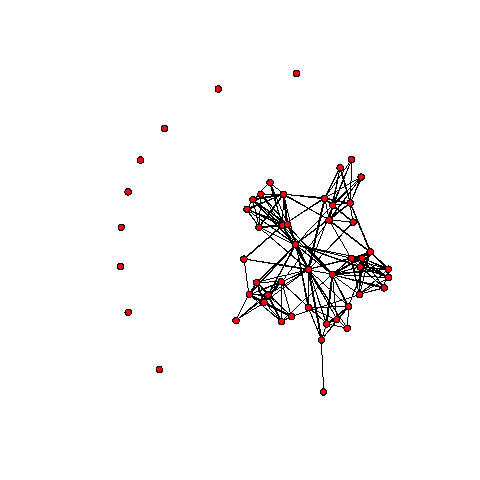
\includegraphics[scale=0.23]{pictures/m1_19_nework.png}
    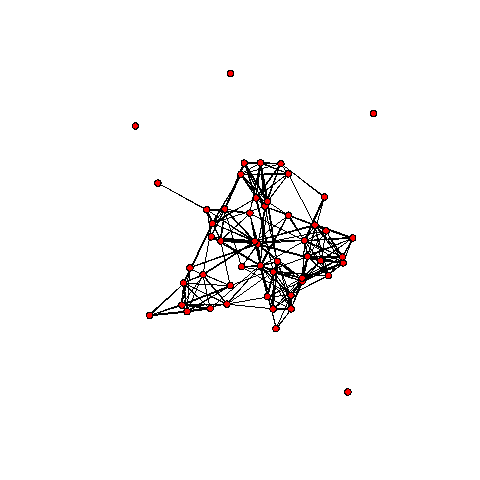
\includegraphics[scale=0.23]{pictures/w1_19_nework.png}
    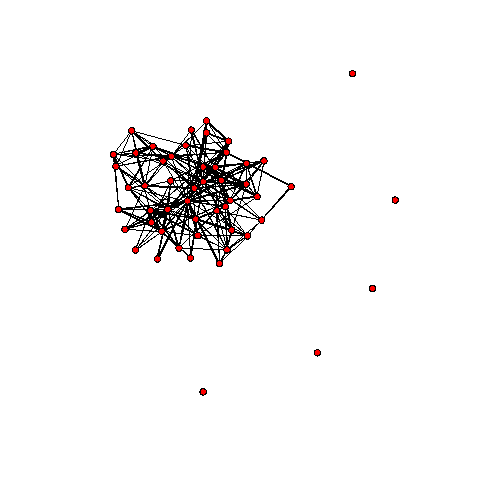
\includegraphics[scale=0.23]{pictures/f1_19_nework.png}
    \caption{Sequence 1}
    % \label{fig:ls}
    \end{center}
\end{figure}
\begin{figure}[h]
    \begin{center}
    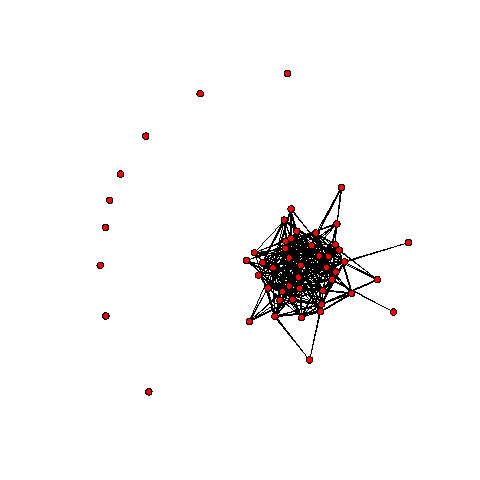
\includegraphics[scale=0.23]{pictures/m2_19_nework.png}
    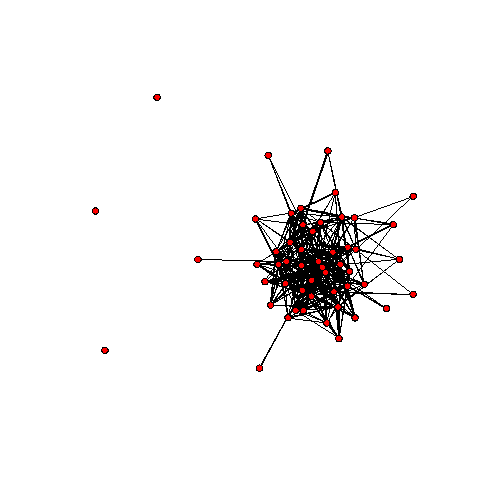
\includegraphics[scale=0.23]{pictures/w2_19_nework.png}
    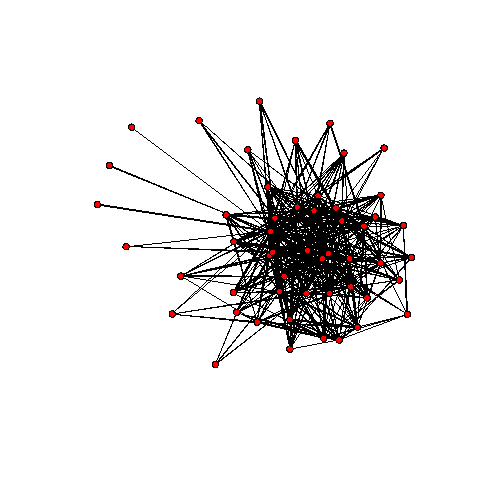
\includegraphics[scale=0.23]{pictures/f2_19_nework.png}
    \caption{Sequence 2}
    % \label{fig:ls}
    \end{center}
\end{figure}
\begin{figure}[h]
    \begin{center}
    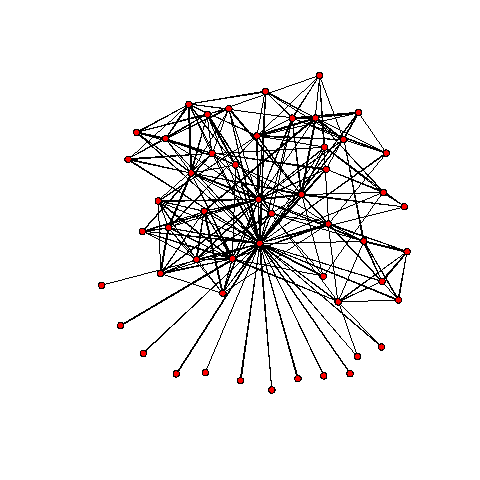
\includegraphics[scale=0.23]{pictures/m3_19_nework.png}
    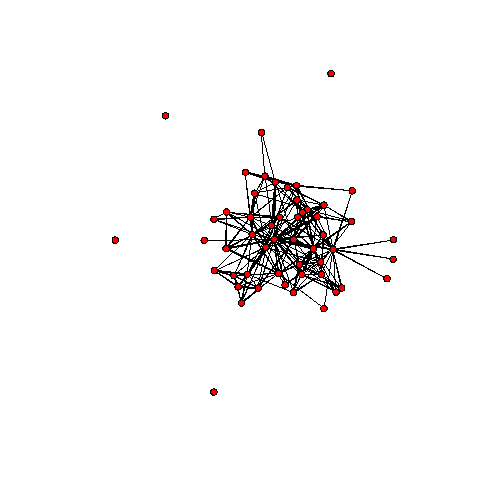
\includegraphics[scale=0.23]{pictures/w3_19_nework.png}
    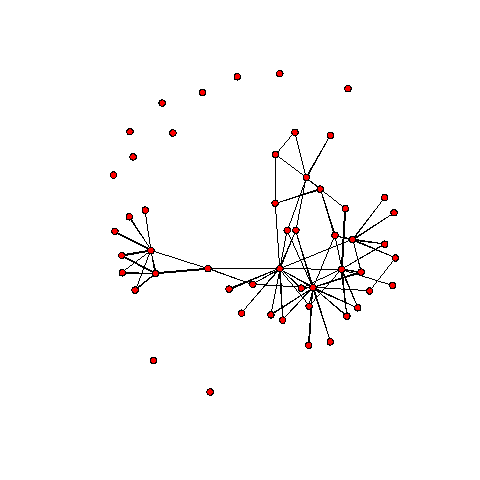
\includegraphics[scale=0.23]{pictures/f3_19_nework.png}
    \caption{Sequence 3}
    % \label{fig:ls}
    \end{center}
\end{figure}
\clearpage

I consider 2 dimentional model as follows.
\[P(Y_t^+=y_t^+|Y_{t-1}=y_{t-1};\theta^+) = \frac{exp((\theta^+)^{T}s(y_t^+, y_{t-1}))}{c(\theta^+, y_{t-1})}\]
\[P(Y_t^-=y_t^-|Y_{t-1}=y_{t-1};\theta^-) = \frac{exp((\theta^-)^{T}s(y_t^-, y_{t-1}))}{c(\theta^-, y_{t-1})}\]
and
\[P(Y_t=y_t|Y_{t-1}=y_{t-1};\theta^+,\theta^-)=P(Y_t^+=y_t^+|Y_{t-1}=y_{t-1};\theta^+) P(Y_t^-=y_t^-|Y_{t-1}=y_{t-1};\theta^-)\]
where
\(s(z_1,z_2)^T=(|z_1|-|z_2|)\)
for $z_1,z_2\in\mathcal{Y}$ with 52 nodes. In other words, the network statistic in the model is
difference of the number of edges for both the formation model and the dissolution model.

I use the ordinary normal prior $p(\theta^+)\sim\mathcal{N}(0,100)$ and $p(\theta^-)\sim\mathcal{N}(0,100)$,
and set the proposal distribution of main chain $\epsilon\sim\mathcal{N}(0,0.0004)$.
The auxiliary chains consist of 1000 iterations and the main chain consists of 50000 iteration.
In this setting, the BSTERGM fitting algorithm run 2400 iterations of main chain per a minute on the intel i7-8700(3.20GHz) CPU.

After generating the chain, I cut first 10000 samples for a burn-in period and thin the sample by 10.
The posterior estimates for each network and histograms are follows.
%mean, sd
\begin{table}[h!]
    \centering
        \begin{tabular}{c | c | c | c }
            Sequence & Parameter & Estimate & Std.Error \\
            \hline \hline
            1 & $\theta^+$ & -2.336387 & 0.1274921 \\
            1 & $\theta^-$ & 1.043077 & 0.1722938 \\
            2 & $\theta^+$ & -1.435648 & 0.1009999 \\
            2 & $\theta^-$ & 0.9332358 & 0.1358161 \\
            3 & $\theta^+$ & -5.02916 & 0.2097569 \\
            3 & $\theta^-$ & 2.225616 & 0.1904817 \\
        \end{tabular}
        \caption{Fitted parameters summary}
        % \label{tab:data}
    \end{table}
\clearpage
%hist
\begin{figure}[h]
    \begin{center}
        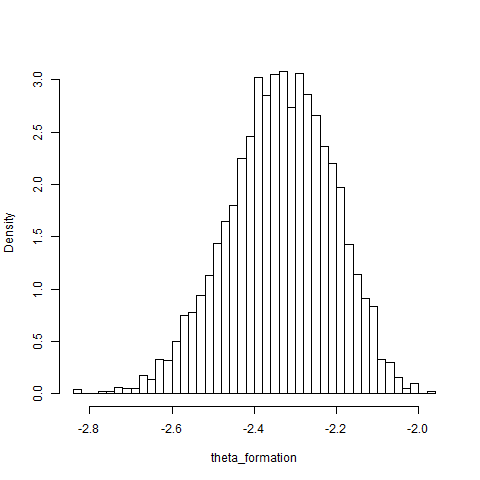
\includegraphics[scale=0.23]{pictures/net1seq_chain1_BSTERGM_formation_histogram.png}
        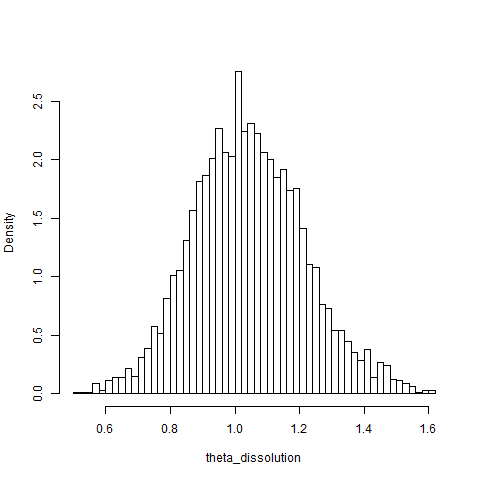
\includegraphics[scale=0.23]{pictures/net1seq_chain1_BSTERGM_dissolution_histogram.png}
    \caption{Sequence 1, left: formation, right: dissolution}
    % \label{fig:ls}
    \end{center}
\end{figure}

\begin{figure}[h]
    \begin{center}
        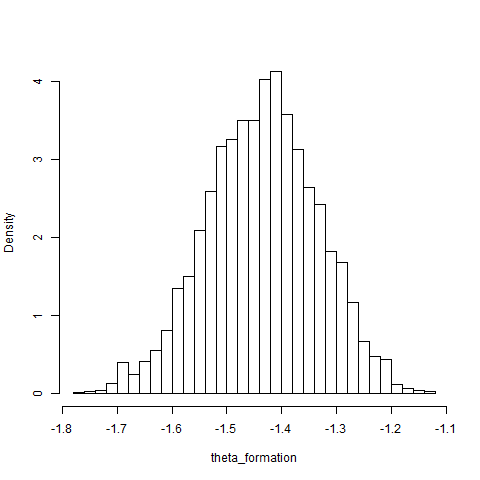
\includegraphics[scale=0.23]{pictures/net2seq_chain1_BSTERGM_formation_histogram.png}
        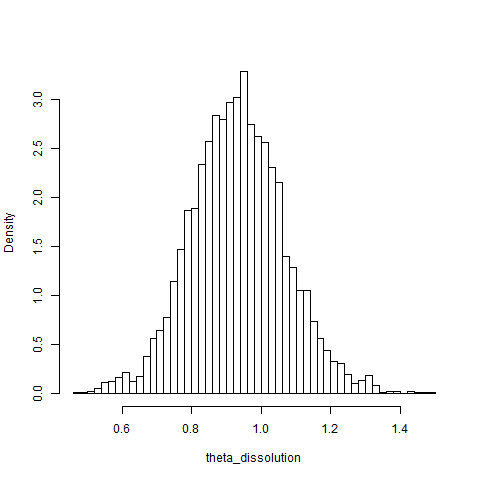
\includegraphics[scale=0.23]{pictures/net2seq_chain1_BSTERGM_dissolution_histogram.png}
    \caption{Sequence 2, left: formation, right: dissolution}
    % \label{fig:ls}
    \end{center}
\end{figure}

\begin{figure}[h]
    \begin{center}
        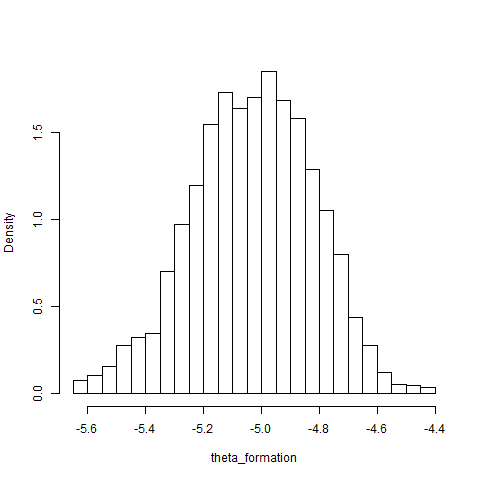
\includegraphics[scale=0.23]{pictures/net3seq_chain1_BSTERGM_formation_histogram.png}
        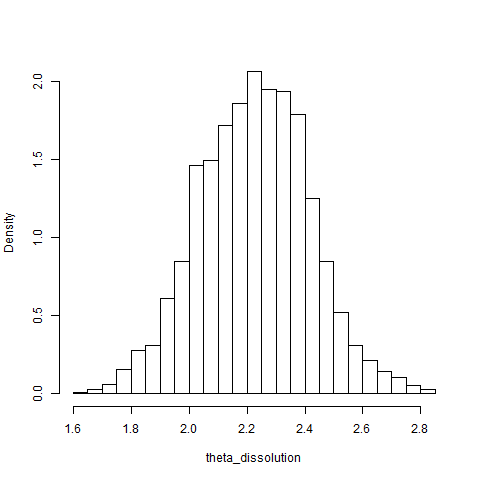
\includegraphics[scale=0.23]{pictures/net3seq_chain1_BSTERGM_dissolution_histogram.png}
    \caption{Sequence 3, left: formation, right: dissolution}
    % \label{fig:ls}
    \end{center}
\end{figure}
\clearpage

For the diagnostics, I attach traceplots and autocorrelation plots.
The autocorrelation of each chain decrease rapidly as lag increases.
Moreover, traceplots shows that the MCMC samples are mixed well.
\begin{figure}[h]
    \begin{center}
        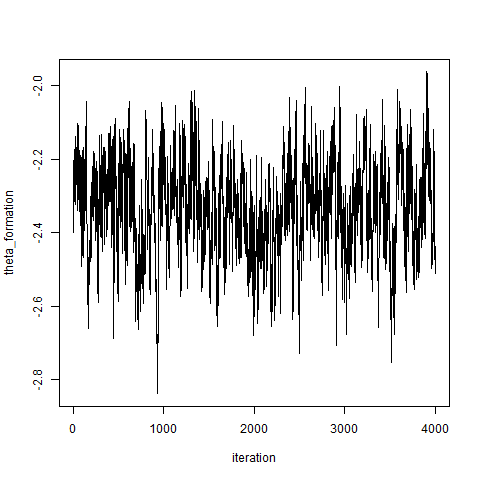
\includegraphics[scale=0.23]{pictures/net1seq_chain1_BSTERGM_formation_traceplot.png}
        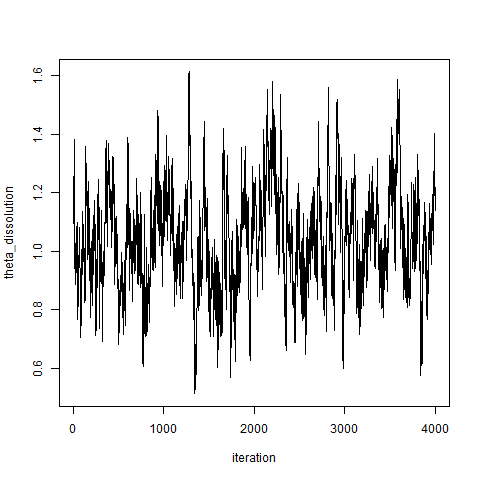
\includegraphics[scale=0.23]{pictures/net1seq_chain1_BSTERGM_dissolution_traceplot.png} \\
        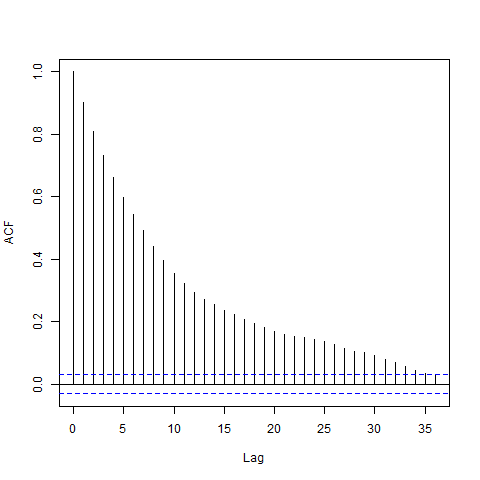
\includegraphics[scale=0.23]{pictures/net1seq_chain1_BSTERGM_formation_acf.png}
        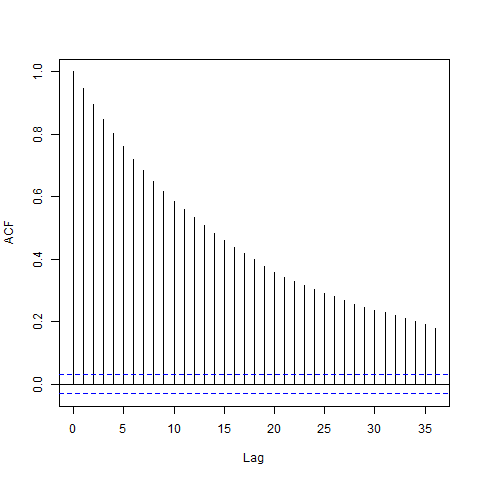
\includegraphics[scale=0.23]{pictures/net1seq_chain1_BSTERGM_dissolution_acf.png}
    \caption{Sequence 1, left: formation, right: dissolution}
    % \label{fig:ls}
    \end{center}
\end{figure}
\begin{figure}[h]
    \begin{center}
        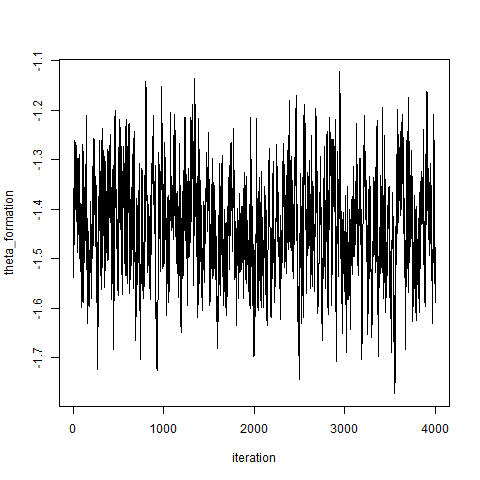
\includegraphics[scale=0.23]{pictures/net2seq_chain1_BSTERGM_formation_traceplot.png}
        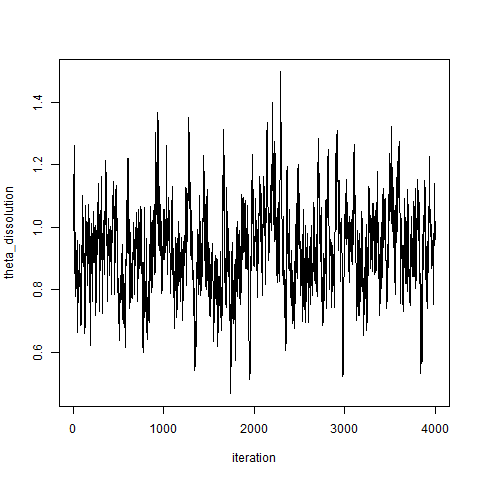
\includegraphics[scale=0.23]{pictures/net2seq_chain1_BSTERGM_dissolution_traceplot.png} \\
        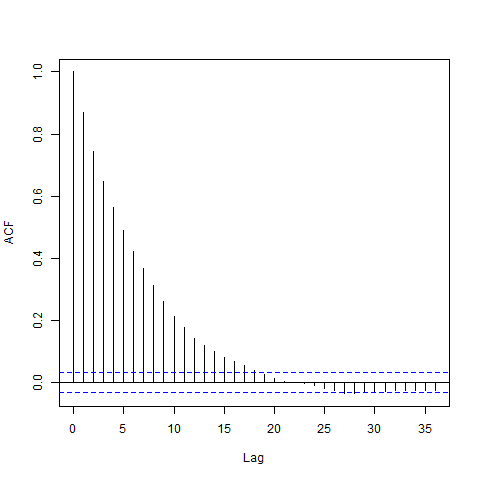
\includegraphics[scale=0.23]{pictures/net2seq_chain1_BSTERGM_formation_acf.png}
        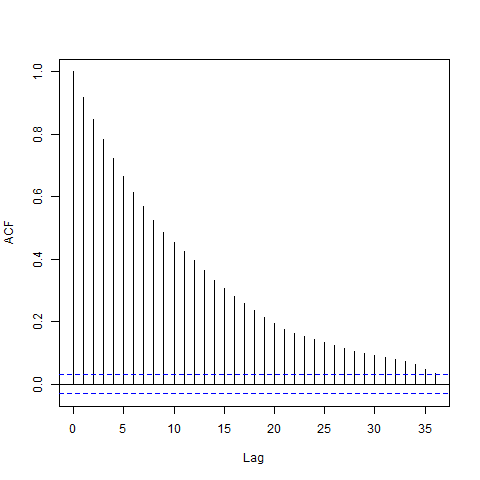
\includegraphics[scale=0.23]{pictures/net2seq_chain1_BSTERGM_dissolution_acf.png}
    \caption{Sequence 2, left: formation, right: dissolution}
    % \label{fig:ls}
    \end{center}
\end{figure}
\begin{figure}[h]
    \begin{center}
        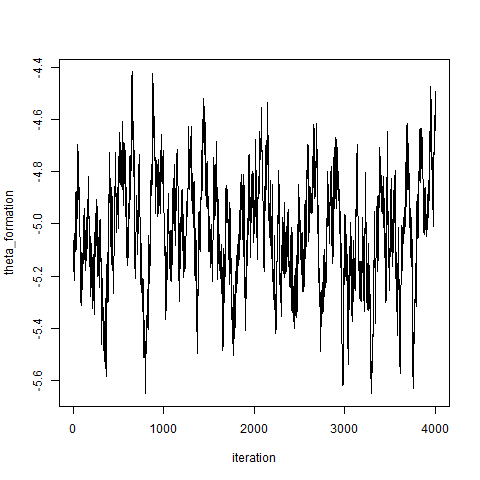
\includegraphics[scale=0.23]{pictures/net3seq_chain1_BSTERGM_formation_traceplot.png}
        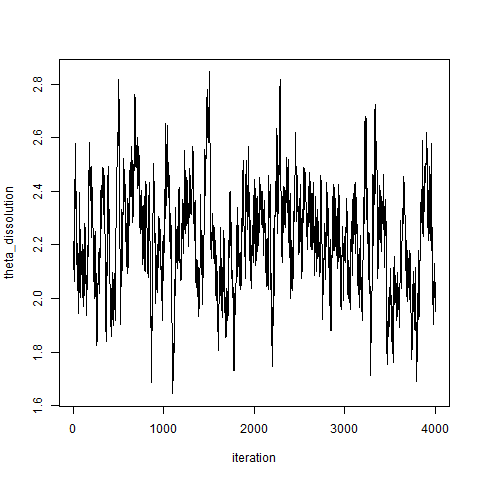
\includegraphics[scale=0.23]{pictures/net3seq_chain1_BSTERGM_dissolution_traceplot.png} \\
        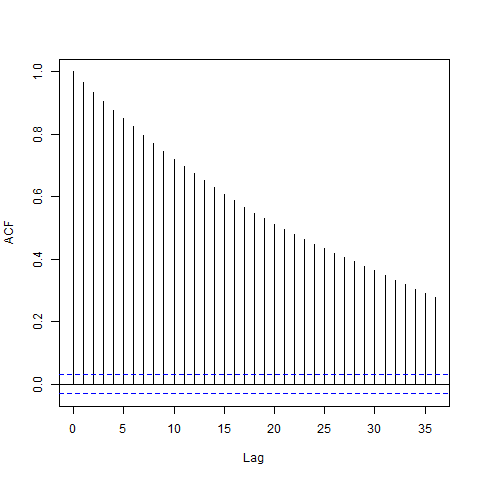
\includegraphics[scale=0.23]{pictures/net3seq_chain1_BSTERGM_formation_acf.png}
        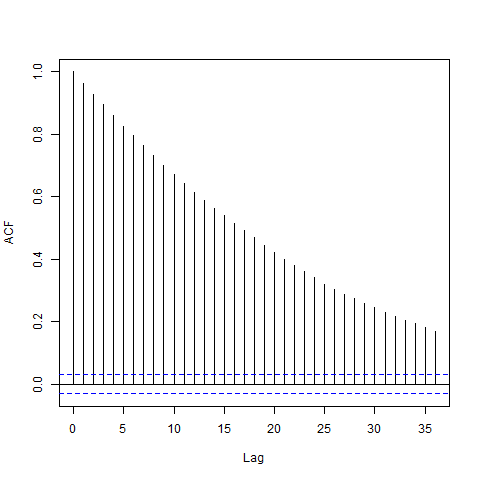
\includegraphics[scale=0.23]{pictures/net3seq_chain1_BSTERGM_dissolution_acf.png}
    \caption{Sequence 3, left: formation, right: dissolution}
    % \label{fig:ls}
    \end{center}
\end{figure}
\clearpage
In addition, as a procedure of diagnostics for auxiliary chains,
here are traceplots of the number of edges in last auxiliary chain.
They shows that all chains are not degenerated at last parameter point during the iterations of auxiliary chain.

%lastsampler
\begin{figure}[h]
    \begin{center}
        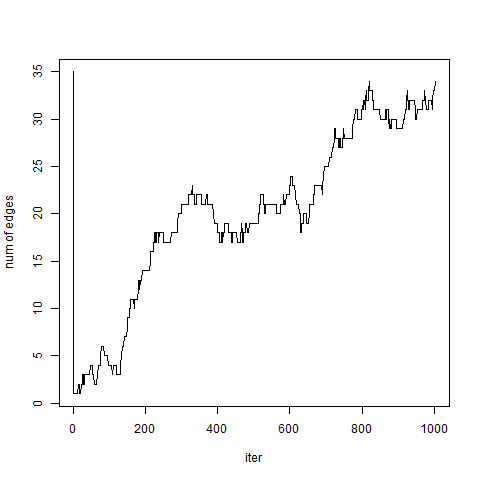
\includegraphics[scale=0.23]{pictures/net1seq_chain1_lastsampler_num_edges.png}
        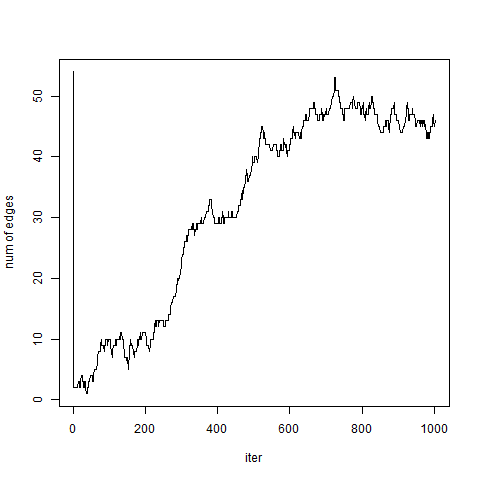
\includegraphics[scale=0.23]{pictures/net2seq_chain1_lastsampler_num_edges.png}
        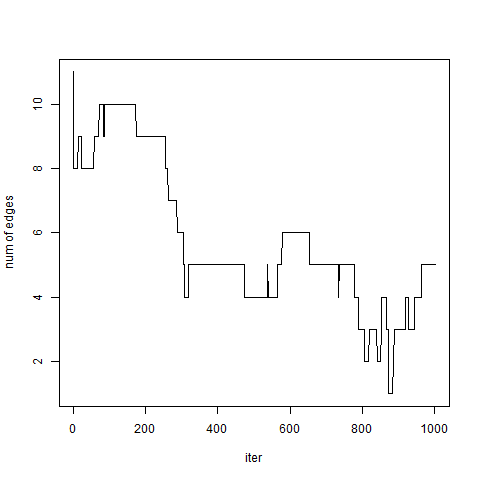
\includegraphics[scale=0.23]{pictures/net3seq_chain1_lastsampler_num_edges.png}
    \caption{Sequence 1, left: formation, right: dissolution}
    % \label{fig:ls}
    \end{center}
\end{figure}
\clearpage


Finally, I append the results of goodness of fit.
Compare observed (true) value with quantiles of simulated values of parts of sufficient network statistics,
generated by the goodness of fit algorithm.
Since this example has simply just two edge terms, and since the BSTERGMs share same parameter
for each network statistics but values of network statistics are different at each time point,
the sufficient statistics do not fitted perfectly to observed networks' values.
However, the tendency of simulated values goes with the observed values.

\begin{table}[h!]
    \centering
        \begin{tabular}{c| c | c | c | c |c |c |c |c }
            Sequence& timelag & netstat & obs & q0.1 & q0.25 & q0.5 & q0.75 & q0.9 \\
            \hline \hline
            1 & 1-2 & $D_0$ & 4 &  0& 0& 0& 1& 1 \\
            1 & 1-2 & $D_1$ & 1 &  0& 0& 1& 2& 3 \\
            1 & 1-2 & $D_2$ & 0 &  1& 1& 2& 3& 4 \\
            1 & 1-2 & $D_3$ & 3 &  1& 2& 3& 4& 5 \\
            1 & 1-2 & $D_4$ & 1 &  1& 2& 3& 4& 6 \\
            1 & 1-2 & $D_5$ & 3 &  2& 3& 4& 5& 7 \\
            1 & 1-2 & $D_6$ & 3 &  2& 3& 5& 6& 8 \\
            1 & 1-2 & $D_7$ & 5 &  3& 4& 5& 7& 9 \\
            1 & 1-2 & $D_8$ & 9 &  3& 4& 6& 7& 9 \\
            1 & 1-2 & $D_9$ & 5 &  3& 4& 6& 7& 9 \\
            1 & 1-2 & $D_{10}$ & 4 &  2& 3& 5& 6& 8 \\
            1 & 1-2 & $D_{11}$ & 4 &  1& 2& 4& 5& 6 \\
            1 & 1-2 & $D_{12}$ & 4 &  0& 1& 2& 3& 5 \\
            1 & 1-2 & $D_{13}$ & 2 &  0& 1& 1& 2& 3 \\
            1 & 1-2 & $D_{14}$ & 1 &  0& 0& 1& 1& 2 \\
            1 & 1-2 & $D_{15}$ & 0 &  0& 0& 0& 1& 2 \\
            1 & 1-2 & $P_0$ & 8 &  25& 28& 33& 37& 42 \\
            1 & 1-2 & $P_1$ & 10 & 29& 33& 38& 43& 48 \\
            1 & 1-2 & $P_2$ & 29 & 30& 33& 38& 43& 47 \\
            1 & 1-2 & $P_3$ & 27 & 28& 32& 36& 40& 44 \\
            1 & 1-2 & $P_4$ & 13 & 19& 23& 28& 32& 37 \\
            1 & 1-2 & $P_5$ & 37 &  9& 13& 17& 22& 26 \\
            1 & 1-2 & $P_6$ & 40 &  3& 5& 8& 11& 15 \\
            1 & 1-2 & $P_7$ & 20 &  3& 4& 5& 7& 9 \\
            1 & 1-2 & $P_8$ & 20 &  0& 1& 3& 5& 7 \\
            1 & 1-2 & $|y_2|$ & 212 &  186& 194& 204& 214& 223 \\
        \end{tabular}
        \caption{GOF: sequence 1 (1)}
        % \label{tab:data}
    \end{table}
\clearpage
\begin{table}[h!]
    \centering
        \begin{tabular}{c| c | c | c | c |c |c |c |c }
            Sequence& timelag & netstat & obs & q0.1 & q0.25 & q0.5 & q0.75 & q0.9 \\
            \hline \hline
            1 & 2-3 & $D_0$ & 5 &  0& 0& 0& 0& 1 \\
            1 & 2-3 & $D_1$ & 0 &  0& 0& 0& 1& 2 \\
            1 & 2-3 & $D_2$ & 2 &  0& 0& 1& 2& 2 \\
            1 & 2-3 & $D_3$ & 1 &  0& 1& 2& 2& 3 \\
            1 & 2-3 & $D_4$ & 2 &  1& 1& 2& 3& 4 \\
            1 & 2-3 & $D_5$ & 5 &  1& 2& 3& 4& 5 \\
            1 & 2-3 & $D_6$ & 2 &  1& 3& 4& 5& 7 \\
            1 & 2-3 & $D_7$ & 3 &  2& 4& 5& 7& 8 \\
            1 & 2-3 & $D_8$ & 8 &  3& 4& 6& 7& 8 \\
            1 & 2-3 & $D_9$ & 4 &  3& 5& 6& 8& 9 \\
            1 & 2-3 & $D_{10}$ & 4 &  3& 4& 5& 7& 9 \\
            1 & 2-3 & $D_{11}$ & 5 &  2& 3& 5& 6& 8 \\
            1 & 2-3 & $D_{12}$ & 1 &  1& 2& 4& 5& 6 \\
            1 & 2-3 & $D_{13}$ & 3 &  1& 2& 2& 4& 5 \\
            1 & 2-3 & $D_{14}$ & 0 &  0& 1& 2& 3& 4 \\
            1 & 2-3 & $D_{15}$ & 1 &  0& 0& 1& 2& 3 \\
            1 & 2-3 & $P_0$ & 11 & 20& 24& 28& 32& 37 \\
            1 & 2-3 & $P_1$ & 12 & 32& 36& 41& 47& 51 \\
            1 & 2-3 & $P_2$ & 23 & 35& 39& 44& 49& 53 \\
            1 & 2-3 & $P_3$ & 52 & 32& 35& 40& 45& 49 \\
            1 & 2-3 & $P_4$ & 39 & 24& 28& 33& 37& 42 \\
            1 & 2-3 & $P_5$ & 24 & 13& 18& 22& 27& 32 \\
            1 & 2-3 & $P_6$ & 21 &  6& 9& 12& 17& 21 \\
            1 & 2-3 & $P_7$ & 20 &  2& 3& 5& 8& 12 \\
            1 & 2-3 & $P_8$ & 13 &  0& 1& 2& 4& 6 \\
            1 & 2-3 & $|y_3|$ & 227 &  213& 222& 232& 243& 253 \\
        \end{tabular}
        \caption{GOF: sequence 1 (2)}
        % \label{tab:data}
    \end{table}
\clearpage

\begin{table}[h!]
    \centering
        \begin{tabular}{c| c | c | c | c |c |c |c |c }
            Sequence& timelag & netstat & obs & q0.1 & q0.25 & q0.5 & q0.75 & q0.9 \\
            \hline \hline
            2 & 1-2 & $D_0$ & 3 &  0& 0& 0& 0& 0 \\
            2 & 1-2 & $D_1$ & 2 &  0& 0& 0& 0& 0 \\
            2 & 1-2 & $D_2$ & 4 &  0& 0& 0& 0& 1 \\
            2 & 1-2 & $D_3$ & 1 &  0& 0& 0& 1& 1 \\
            2 & 1-2 & $D_4$ & 3 &  0& 0& 1& 1& 2 \\
            2 & 1-2 & $D_5$ & 0 &  0& 0& 1& 2& 3 \\
            2 & 1-2 & $D_6$ & 0 &  0& 1& 2& 3& 4 \\
            2 & 1-2 & $D_7$ & 1 &  0& 1& 2& 3& 4 \\
            2 & 1-2 & $D_8$ & 4 &  1& 1& 2& 4& 5 \\
            2 & 1-2 & $D_9$ & 1 &  1& 1& 2& 3& 5 \\
            2 & 1-2 & $D_{10}$ & 3 &  1& 2& 3& 4& 5 \\
            2 & 1-2 & $D_{11}$ & 1 &  1& 2& 2& 4& 5 \\
            2 & 1-2 & $D_{12}$ & 1 &  1& 2& 3& 4& 5 \\
            2 & 1-2 & $D_{13}$ & 2 &  1& 2& 3& 4& 5 \\
            2 & 1-2 & $D_{14}$ & 3 &  1& 2& 3& 4& 5 \\
            2 & 1-2 & $D_{15}$ & 1 &  1& 2& 3& 4& 6 \\
            2 & 1-2 & $D_{16}$ & 1 &  1& 2& 3& 4& 6 \\
            2 & 1-2 & $D_{17}$ & 3 &  1& 2& 2& 4& 6 \\
            2 & 1-2 & $D_{18}$ & 2 &  1& 2& 3& 4& 6 \\
            2 & 1-2 & $D_{19}$ & 2 &  1& 2& 3& 4& 5 \\
            2 & 1-2 & $D_{20}$ & 2 &  1& 2& 3& 4& 5 \\
            2 & 1-2 & $D_{21}$ & 2 &  0& 1& 2& 3& 4 \\
            2 & 1-2 & $P_4$ & 21 & 33& 38& 43& 48& 52 \\
            2 & 1-2 & $P_5$ & 28 & 35& 38& 43& 48& 54 \\
            2 & 1-2 & $P_6$ & 31 & 33& 37& 42& 47& 52 \\
            2 & 1-2 & $P_7$ & 31 & 28& 32& 37& 43& 48 \\
            2 & 1-2 & $P_8$ & 32 & 21& 25& 31& 36& 41 \\
            2 & 1-2 & $P_9$ & 23 & 14& 18& 23& 29& 33 \\
            2 & 1-2 & $P_{10}$ & 27 & 8& 12& 16& 21& 26 \\
            2 & 1-2 & $P_{11}$ & 21 & 4& 7& 10& 14& 19 \\
            2 & 1-2 & $|y_2|$ & 342 &  344& 356& 370& 387& 400 \\
        \end{tabular}
        \caption{GOF: sequence 2 (1)}
        % \label{tab:data}
    \end{table}
\clearpage
\begin{table}[h!]
    \centering
        \begin{tabular}{c| c | c | c | c |c |c |c |c }
            Sequence& timelag & netstat & obs & q0.1 & q0.25 & q0.5 & q0.75 & q0.9 \\
            \hline \hline
            2 & 2-3 & $D_0$ & 0 &  0& 0& 0& 0& 0 \\
            2 & 2-3 & $D_1$ & 3 &  0& 0& 0& 0& 0 \\
            2 & 2-3 & $D_2$ & 1 &  0& 0& 0& 0& 0 \\
            2 & 2-3 & $D_3$ & 2 &  0& 0& 0& 0& 1 \\
            2 & 2-3 & $D_4$ & 2 &  0& 0& 0& 1& 2 \\
            2 & 2-3 & $D_5$ & 1 &  0& 0& 1& 1& 2 \\
            2 & 2-3 & $D_6$ & 1 &  0& 0& 1& 2& 3 \\
            2 & 2-3 & $D_7$ & 2 &  0& 1& 2& 3& 4 \\
            2 & 2-3 & $D_8$ & 1 &  1& 1& 2& 3& 4 \\
            2 & 2-3 & $D_9$ & 1 &  1& 1& 2& 3& 5 \\
            2 & 2-3 & $D_{10}$ & 3 &  1& 2& 3& 4& 5 \\
            2 & 2-3 & $D_{11}$ & 2 &  1& 1& 2& 4& 5 \\
            2 & 2-3 & $D_{12}$ & 2 &  1& 2& 4& 5& 6 \\
            2 & 2-3 & $D_{13}$ & 3 &  1& 2& 3& 4& 5 \\
            2 & 2-3 & $D_{14}$ & 2 &  1& 2& 3& 4& 5 \\
            2 & 2-3 & $D_{15}$ & 0 &  1& 2& 3& 4& 5 \\
            2 & 2-3 & $D_{16}$ & 3 &  1& 2& 3& 4& 5 \\
            2 & 2-3 & $D_{17}$ & 1 &  1& 2& 2& 4& 5 \\
            2 & 2-3 & $D_{18}$ & 0 &  1& 2& 3& 4& 5 \\
            2 & 2-3 & $D_{19}$ & 3 &  1& 2& 3& 4& 5 \\
            2 & 2-3 & $D_{20}$ & 2 &  1& 2& 3& 4& 5 \\
            2 & 2-3 & $D_{21}$ & 0 &  1& 1& 2& 3& 4 \\
            2 & 2-3 & $P_4$ & 6 & 35& 29& 44& 48& 53 \\
            2 & 2-3 & $P_5$ & 27 & 34& 38& 42& 48& 53 \\
            2 & 2-3 & $P_6$ & 34 & 35& 39& 44& 49& 53 \\
            2 & 2-3 & $P_7$ & 25 & 33& 36& 41& 46& 50 \\
            2 & 2-3 & $P_8$ & 27 & 28& 32& 27& 42& 47 \\
            2 & 2-3 & $P_9$ & 39 & 22& 26& 31& 36& 40 \\
            2 & 2-3 & $P_{10}$ & 24 & 15& 19& 24& 29& 34 \\
            2 & 2-3 & $P_{11}$ & 27 & 10& 14& 18& 23& 27 \\
            2 & 2-3 & $|y_3|$ & 433 &  375& 387& 402& 417& 430 \\
        \end{tabular}
        \caption{GOF: sequence 2 (2)}
        % \label{tab:data}
    \end{table}
\clearpage


\begin{table}[h!]
    \centering
        \begin{tabular}{c| c | c | c | c |c |c |c |c }
            Sequence& timelag & netstat & obs & q0.1 & q0.25 & q0.5 & q0.75 & q0.9 \\
            \hline \hline
            3 & 1-2 & $D_0$ & 4 &  0& 0& 0& 1& 2 \\
            3 & 1-2 & $D_1$ & 4 &  6& 7& 8& 9& 10 \\
            3 & 1-2 & $D_2$ & 3 &  1& 2& 3& 4& 5 \\
            3 & 1-2 & $D_3$ & 1 &  0& 0& 1& 1& 2 \\
            3 & 1-2 & $D_4$ & 2 &  0& 1& 1& 2& 3 \\
            3 & 1-2 & $D_5$ & 7 &  1& 2& 3& 4& 5 \\
            3 & 1-2 & $D_6$ & 4 &  3& 4& 5& 7& 8 \\
            3 & 1-2 & $D_7$ & 3 &  3& 4& 5& 6& 7 \\
            3 & 1-2 & $D_8$ & 4 &  2& 3& 4& 5& 6 \\
            3 & 1-2 & $D_9$ & 6 &  2& 3& 4& 5& 6 \\
            3 & 1-2 & $D_{10}$ & 0 &  2& 3& 4& 5& 6 \\
            3 & 1-2 & $D_{11}$ & 6 &  2& 3& 4& 5& 6 \\
            3 & 1-2 & $D_{12}$ & 2 &  1& 1& 2& 3& 4 \\
            3 & 1-2 & $D_{13}$ & 1 &  0& 1& 1& 2& 3 \\
            3 & 1-2 & $D_{14}$ & 0 &  0& 1& 1& 2& 3 \\
            3 & 1-2 & $D_{15}$ & 0 &  0& 0& 1& 1& 2 \\
            3 & 1-2 & $P_0$ & 7 & 9& 10& 12& 13& 14 \\
            3 & 1-2 & $P_1$ & 22 & 12& 14& 17& 20& 23 \\
            3 & 1-2 & $P_2$ & 21 & 15& 18& 21& 24& 27 \\
            3 & 1-2 & $P_3$ & 42 & 23& 27& 30& 34& 37 \\
            3 & 1-2 & $P_4$ & 24 & 25& 29& 32& 36& 40 \\
            3 & 1-2 & $P_5$ & 32 & 22& 25& 29& 33& 37 \\
            3 & 1-2 & $P_6$ & 14 & 15& 18& 21& 23& 26 \\
            3 & 1-2 & $P_7$ & 9 & 12& 14& 17& 19& 22 \\
            3 & 1-2 & $P_8$ & 14 & 7& 9& 12& 14& 16 \\
            3 & 1-2 & $P_9$ & 6 &  3& 5& 7& 9& 11 \\
            3 & 1-2 & $P_10$ & 1 &  1& 2& 3& 4& 5 \\
            3 & 1-2 & $|y_2|$ & 196 &  198& 201& 206& 209& 213 \\
        \end{tabular}
        \caption{GOF: sequence 3 (1)}
        % \label{tab:data}
    \end{table}
\clearpage
\begin{table}[h!]
    \centering
        \begin{tabular}{c| c | c | c | c |c |c |c |c }
            Sequence& timelag & netstat & obs & q0.1 & q0.25 & q0.5 & q0.75 & q0.9 \\
            \hline \hline
            3 & 2-3 & $D_0$ & 11 &  2& 3& 3& 4& 4 \\
            3 & 2-3 & $D_1$ & 11 &  2& 3& 4& 5& 6 \\
            3 & 2-3 & $D_2$ & 12 &  2& 2& 3& 4& 5 \\
            3 & 2-3 & $D_3$ & 9 &  1& 1& 2& 3& 3 \\
            3 & 2-3 & $D_4$ & 2 &  2& 2& 3& 4& 5 \\
            3 & 2-3 & $D_5$ & 1 &  4& 5& 6& 7& 8 \\
            3 & 2-3 & $D_6$ & 0 &  2& 3& 4& 6& 7 \\
            3 & 2-3 & $D_7$ & 2 &  2& 3& 4& 5& 6 \\
            3 & 2-3 & $D_8$ & 1 &  2& 3& 4& 5& 6 \\
            3 & 2-3 & $D_9$ & 0 &  2& 3& 4& 5& 6 \\
            3 & 2-3 & $D_{10}$ & 1 &  1& 2& 3& 4& 5 \\
            3 & 2-3 & $D_{11}$ & 0 &  1& 2& 3& 4& 5 \\
            3 & 2-3 & $D_{12}$ & 0 &  0& 1& 1& 2& 3 \\
            3 & 2-3 & $D_{13}$ & 0 &  0& 0& 0& 1& 2 \\
            3 & 2-3 & $D_{14}$ & 1 &  0& 0& 0& 0& 1 \\
            3 & 2-3 & $D_{15}$ & 1 &  0& 0& 0& 1& 1 \\
            3 & 2-3 & $P_0$ & 36 & 8& 10& 12& 14& 16 \\
            3 & 2-3 & $P_1$ & 26 & 20& 22& 25& 28& 31 \\
            3 & 2-3 & $P_2$ & 4 & 23& 26& 30& 34& 37 \\
            3 & 2-3 & $P_3$ & 0 & 29& 33& 37& 40& 44 \\
            3 & 2-3 & $P_4$ & 1 & 21& 24& 27& 31& 34 \\
            3 & 2-3 & $P_5$ & 0 & 16& 18& 22& 25& 28 \\
            3 & 2-3 & $P_6$ & 0 &  8& 10& 12& 14& 16 \\
            3 & 2-3 & $P_7$ & 1 &  6& 7& 9& 11& 13 \\
            3 & 2-3 & $P_8$ & 0 &  3& 4& 6& 8& 10 \\
            3 & 2-3 & $P_9$ & 0 &  1& 1& 2& 4& 5 \\
            3 & 2-3 & $P_10$ & 0 &  0& 1& 1& 2& 3 \\
            3 & 2-3 & $|y_3|$ & 227 &  180& 183& 187& 190& 193 \\
        \end{tabular}
        \caption{GOF: sequence 3 (2)}
        % \label{tab:data}
    \end{table}
\clearpage


%GOF table

\section{Summary and Discussion}
In this paper, I have proposed the Bayesian STERGMs for a sequence of networks
and a framework for statistical estimation and inference using the standard Bayesian approach for the model.
I also have shown a application of the BSTERGMs. %more add

Since the models are based on ERGMs, it can be extended to more general networks
including a variety of network statistics.
Moreover, the model can be applied to weighted graph and use the weights as covariates of the model.
Plus, the BSTERGMs are using the exchange algorithm, so it is flexible enough to be integrated
with other methods to help the MCMC chains to converge and run faster.
For example, the 'tie no tie'(TNT) algorithm used by ergm package (\cite{RN100}) can be applied to
enhance the performance of the auxiliary chain of the BSTERGMs.

A modeling by the BSTERGMs for large networks is possible,
but a problem of computational inefficiency rises.
If given observed network has lots of nodes, the estimation algorithm for the BSTERGM needs 
huge number of auxiliary chain itertation to sample a proper exchange network at a given parameter point.
In addition, the calculation of network statistics in the model cause another problem for large networks,
especially when the model has network statistics that high complexity of computation.
For example, statistics based on edgewise shared partner distributions needs $O(n^3)$,
so computation cost increases rapidly as the number of nodes $n$ grows and
the auxiliary chains become bottlenecks of the whole computation procedure.

Another important issue related in the BSTERGMs is degeneracy as I have mentioned at the section of model diagnostics.
The BSTERGMs are very sensitive to the initial point of main MCMC chain, so
searching a region for non-degenerate initial parameter point in the parameter space is very important.
Often, however, the work finding the region is too difficult for the BSTERGMs,
partly because of the high number of parameters in the models.
Since the BSTERGMs has two parts for $\theta^-, \theta^+$ in the setting of the models by the their definition,
the dimension of parameter space increases easily although each formation and dissolution model does not have
too many terms respectively.
What makes the situation worse is not only the high dimension of parameter space but also the shape of convergent region of the parameter.
In many case, the region is geometrically curved due to an implicit relation between several network statistics in the models
and interaction between the formation model and the dissolution model.
Thus, the MCMC algorithm may fail to exploring the whole parameter space, especially when the space has high dimension,
and suffer non-convergence problem.
Imposing some model level constraint or using special prior may be a remedy,
but finding the proper constraint or the prior distribution will often be a more difficult problem than original one.
Thus, further research is needed to resolve these issues.


\begin{frame}{Supplements}
    You can find the C++ implementation (using Armadilo: see http://arma.sourceforge.net/)
    \\ of BSTERGM fitting, diagnostic, and GOF algorithms
    \\ at my Github page: https://github.com/letsjdosth/BayesianSTERGM.
\end{frame}



\nocite{*}
\bibliographystyle{apalike}
\bibliography{doc.bib}

\end{document}
